\documentclass[10pt,twocolumn,letterpaper]{article}

\usepackage[letterpaper, top=1in, bottom=1in, left=0.75in, right=0.75in]{geometry}
\usepackage[T1]{fontenc}
\usepackage[utf8]{inputenc}
\usepackage[english]{babel}
\usepackage{lmodern}
\usepackage{microtype}

\usepackage{amsmath}
\usepackage{amssymb}
\usepackage{booktabs}
\usepackage{multirow}
\usepackage{url}
\usepackage{xurl}
\usepackage[hidelinks,breaklinks=true]{hyperref}
\usepackage{graphicx}
\usepackage{tabularx}
\usepackage{array}
\usepackage{enumitem}
\usepackage{xcolor}
\usepackage{tikz}
\usepackage{pgfplots}
\pgfplotsset{compat=1.18}
\usetikzlibrary{patterns,calc,decorations.pathreplacing}
\usepackage{draftwatermark}
\SetWatermarkText{DRAFT}
\SetWatermarkScale{1.2}
\SetWatermarkColor[gray]{0.92}
\setlength{\parskip}{0pt}
\setlength{\parsep}{0pt}
\setlength{\columnsep}{0.25in}

\title{\Large\textbf{Unmonitored by Design: A Longitudinal Measurement Study\\of Governance Failure in the Web PKI}\\[0.5em]
\normalsize\textit{Working Draft --- Not for citation or distribution}}

\author{
Research\\
\textit{Systematic Reasoning, Inc.}\\
\texttt{info@systematicreasoning.com}
}

\date{}

\begin{document}

\maketitle

\begin{abstract}
The Web PKI enforces compliance through \textit{Public Disclosure with Active
Scrutiny}: CAs disclose failures publicly and browser root programs are expected
to scrutinize and press for remediation. We present the first longitudinal
measurement of whether this model functions. Using the \textit{WebPKI
Observatory}---an open-source pipeline synthesizing CT logs, CCADB root
metadata (335 roots, 89 owners), and 1,428 Bugzilla compliance incidents with
6,036 classified comments (2014--2026)---we establish four findings.
(1)~Issuance follows a tight inverse power law: PPM~$\propto$~share$^{-0.87}$
($r=-0.94$), placing tail CA failure densities $1{,}130\times$ the head while
both hold identical trust.
(2)~Bugzilla oversight coverage has declined for both Chrome and Mozilla
through key-person dependency without institutional redundancy, compounded
by the 2022 Chrome Root Program independence launch, 2022--2023 industry
workforce reductions, and the 2023 eIDAS Article~45 legal challenge to
root program autonomy. Both programs now sit below 20\% Bugzilla coverage
while CA self-filing has surged to 46.1\% of incidents in 2025 and
43.2\% in 2026~Q1---signaling the ecosystem internalizing the monitoring
function---and automated CT linting accounts for 17.3\% all-time.
Apple's rising participation (14.7\% in 2026~Q1) and the 2024 Entrust
distrust demonstrate the enforcement function remains capable on
sufficiently documented cases---a standard that in practice requires a
median 1,185 days and in 73\% of events an accumulated pattern of
failures rather than a single catastrophic trigger.
(3)~The Microsoft Root Store constitutes a structurally separate oversight
environment: zero governance comments on other CAs' incidents across 12 years,
142 exclusive roots with no cross-program oversight, and four CAs distrusted
by all peers still trusted today.
(4)~The transition to 47-day maximum certificate validity---with GoDaddy
(13.0\% share) and IdenTrust (1.0\%) at 145 and 130 days respectively---will
require automation from subscribers who have not yet built it, at a moment
when the Bugzilla oversight coverage rate is at its lowest measured level.
\end{abstract}

\section{Introduction}

The security of HTTPS traffic does not ultimately rest on cryptographic
primitives. It rests on the willingness and capacity of browser vendors to
enforce compliance among the organizations whose root certificates they
distribute. Cryptographic primitives can be verified automatically. CA
compliance cannot. When a CA issues certificates for unvalidated domains,
fails to revoke on schedule, or conceals an infrastructure compromise, the
only remedy the ecosystem possesses is public disclosure followed by
sustained investigative pressure from root programs. The CA/Browser Forum
Baseline Requirements (BRs) exist as written rules, but they carry no
self-executing enforcement mechanism. Enforcement is purely relational.

This paper asks whether that enforcement is happening, and measures what
happens when it is not. We construct, for the first time, a time-indexed
record of root program oversight quality across the full history of the
CA/Browser Forum's public compliance process---2014 through 2026~Q1---using
automated LLM classification of every governance comment left by browser
vendor staff across 1,428 compliance bugs.

Our findings are structural, not incidental. Both programs that historically
provided the bulk of Bugzilla oversight saw their coverage rates decline
when dominant individual contributors reduced engagement between 2020 and
2022---a shared structural vulnerability, not a judgment on program intent
or quality. The detection function has been substantially assumed by CA
self-monitoring and automated CT infrastructure. The Microsoft Root Store
operates without the cross-program oversight that characterizes the other
three programs. And the 47-day validity transition is forcing automation
requirements onto subscribers who have not yet implemented them, as Bugzilla
coverage reaches its lowest measured level.

The governance model this paper evaluates was designed when fewer than
twenty CAs held trust and a handful of browser engineers could realistically
know them all. The trust surface today comprises 335 roots across 89 CA
owners in a market so concentrated that six organizations issue 93.8\% of
all certificates---while 74 tail CAs hold identical trust with per-certificate
failure rates up to three orders of magnitude higher. A further structural
property sharpens the picture: of 97 CA owners currently trusted by at
least one root store, 36 (37\%) issue zero unexpired certificates. These
CA owners hold browser-trusted roots, carry the same trust anchor as the
largest issuers, generate no CT log record to monitor, file no Bugzilla
incidents to assess, and yet each represents an acquisition or compromise
target with pre-established trust---invisible to the governance mechanisms
that depend on issuance activity to generate signal. Some of these 36
have historical issuance now expired (including CAs operating through
cross-sign arrangements) or are in post-distrust transition periods
where active roots remain in some stores; the issuance-gap finding is
a property of the current observable record, not a claim about
operational intent. The governance model
was not designed for this structure, and the data shows where the gap is.

\textbf{Contributions.}
\begin{itemize}[noitemsep,topsep=2pt]
\item The first empirical evaluation of whether a governance model designed
  for a small closed community of CAs still functions at the current scale
  of 335 roots and 89 owners---using the first longitudinal time-series of
  root program oversight quality (coverage rate metric,
  Section~\ref{sec:coverage}), derived from LLM-classified public governance
  records.
\item Measurement of the shared structural vulnerability in Chrome and
  Mozilla's coverage rates---dominant individual contributor dependency
  without redundancy---with quarterly granularity distinguishing the two
  episodes by timing and context
  (Figures~\ref{fig:quarterly},~\ref{fig:concentration}, Section~\ref{sec:keyperson}).
\item Quantification of the PPM inverse power law ($r=-0.94$, robust across
  normalizations) and its implication for tail CA risk allocation
  (Section~\ref{sec:powerlaw}).
\item Measurement of the discovery channel transition: CA self-filing
  has surged to 46.1\% of incidents in 2025 (43.2\% in 2026~Q1) while
  automated CT infrastructure accounts for 17.3\% all-time and root
  programs initiate only 4.1\%---a structural shift in who detects
  compliance failures (Figure~\ref{fig:discovery}, Section~\ref{sec:discovery}).
\item A structural analysis of Microsoft's governance posture using
  source code-level attribution distinguishing CA operator comments from
  root program governance (Section~\ref{sec:microsoft}).
\item Concrete readiness measurements for the 47-day validity transition
  identifying specific CAs representing 14.0\% of all active certificates
  that will breach the March 2027 100-day threshold (Section~\ref{sec:validity}).
\end{itemize}

The paper proceeds from market structure (Section~\ref{sec:market}: who
holds trust and at what failure density) through oversight measurement
(Section~\ref{sec:oversight}: the decline of root program Bugzilla
engagement, its structural causes, and what is replacing it) to three
stress tests that expose the consequences: the Microsoft Root Store as an
existence proof of zero-oversight operation (Section~\ref{sec:microsoft}),
the distrust record as evidence of what the accountability process produces
under current capacity (Section~\ref{sec:distrust}), and the 47-day
validity transition as a simultaneous demand on oversight capacity arriving
at its lowest measured point (Section~\ref{sec:validity}).
Sections~\ref{sec:microsoft} through~\ref{sec:validity} are not independent
findings; each tests the same governance fragility documented in
Section~\ref{sec:oversight} against a different dimension of the current
ecosystem.

\section{Background}
\label{sec:background}

\subsection{Governance by Public Disclosure}
The CA/Browser Forum (CABF) produces the Baseline Requirements that all
trusted CAs must follow. Compliance is verified through annual WebTrust or
ETSI audits, but audits are annual snapshots. Continuous enforcement depends
on a separate channel: when a CA discovers or is notified of a compliance
failure, it must file a public incident report in the Mozilla Bugzilla CA
Certificate Compliance component. Root program representatives are expected
to engage substantively with these disclosures---pressing for root cause,
scope assessment, and credible remediation---before closing the bug.

This channel has no parallel in other regulated industries. There is no
equivalent of an SEC comment letter or FDA inspection report that root
programs produce. There are no minimum response standards, no staffing
requirements, and no audit of the auditors. Governance is entirely
voluntary, entirely informal, and---as our data shows---entirely dependent
on specific individuals.

\subsection{Certificate Transparency}
CT~\cite{laurie2014}, mandated for Chrome from 2018, provides an
append-only public record of all issued certificates. It transformed the
WebPKI from opaque to measurable, enabling real-time misissuance detection.
Revocation failures---which constitute 21.4\% of incidents in our corpus---
were measured end-to-end by Liu et al.~\cite{liu2015}; CT subsequently
made such failures easier to detect automatically.
CT linting tools operate on public logs to surface encoding errors and
policy violations automatically, without the staffing constraints that
bound human oversight. Their role in incident discovery---and the
structural limits of what certificate-content inspection can reach---are
measured in Section~\ref{sec:discovery}.

\subsection{Related Work}
Durumeric et al.~\cite{durumeric2013} established the baseline measurement
methodology for the HTTPS certificate ecosystem. Clark and van
Oorschot~\cite{clark2013} provide a systematic survey of SSL/HTTPS attack
surfaces and trust model assumptions. VanderSloot et
al.~\cite{vandersloot2017} studied CT's effects on ecosystem transparency.
Liu et al.~\cite{liu2015} measured certificate revocation end-to-end;
Chung et al.~\cite{chung2017} examined OCSP must-staple deployment, both
establishing that revocation mechanisms often fail in practice despite
formal requirements. Felt et al.~\cite{felt2017} and Akhawe and
Felt~\cite{akhawe2013} examined browser security indicators. Amann et
al.~\cite{amann2017} measured the WebPKI's response to the DigiNotar
distrust, establishing that ecosystem improvement after a major CA removal
is measurable and slow. Aas et al.~\cite{aas2019} describe Let's
Encrypt's design and its role in automating certificate issuance. Sun et
al.~\cite{sun2024} examine CT monitoring infrastructure and the role of
third-party monitors. Prior measurement work has treated certificate
properties---key sizes, validity periods, chain structure---as the primary
signal. We differ by treating \textit{institutional behavior}---root program
engagement quality over time---as the primary measurement target, and by
introducing the first longitudinal time-series of that engagement.

The paper's findings also connect to the broader internet governance
literature, though we do not attempt a full survey here. The voluntary,
informal governance model the paper documents is characteristic of
multi-stakeholder internet governance more generally: obligations are
established through consensus processes, enforcement depends on
reputational and relational mechanisms rather than statutory authority,
and participation costs are borne by individuals who internalize a
diffuse public benefit~\cite{mueller2010}. The public goods
framing in Section~\ref{sec:discuss} draws on this literature.
The specific failure mode documented here---key-person concentration
in the absence of minimum participation standards---is a recurring
pattern in voluntary technical governance bodies~\cite{simcoe2012}:
IETF working groups exhibit similar contributor concentration and
participation asymmetry, though systematic longitudinal measurement
of the kind this paper introduces has not previously been applied to
root program oversight.

\section{Observatory Methodology}
\label{sec:methodology}

\subsection{Data Sources and Pipeline}
The WebPKI Observatory~\cite{github} is an open-source pipeline running
daily at 06:00~UTC, producing a versioned JSON dataset and LLM
snapshot~\cite{snapshot}. Data in this paper reflects the March 18, 2026
snapshot. Four primary sources are synthesized:

\noindent\textbf{Certificate Transparency (crt.sh).}
Aggregate unexpired and all-time precertificate counts per CA owner from
CT logs. Attribution uses the root owner, not the issuing CA: certificates
issued through cross-signed intermediates are attributed to the root owner.
All market share and PPM calculations reflect this attribution.

\noindent\textbf{CCADB.}
AllCertificateRecordsCSVFormatv4 providing root certificate metadata, trust
store inclusion per program, and CA owner records for 335 unique included
roots across 89 CA owners. Of these, 317 roots belonging to 96 CA owners
with active certificate issuance are used in the cryptographic posture
analysis (Section~\ref{sec:crypto}).

\noindent\textbf{Mozilla Bugzilla.}
Complete scrape of the CA Certificate Compliance component, 2014--present.
All 1,428 active-CA incident reports with full comment histories. This is the
canonical public record of CA compliance failures and root program responses.
Incidents from CAs subsequently distrusted by all programs are tracked
separately and excluded from primary analysis.

\noindent\textbf{CA/Browser Forum + Chromium Git.}
CABF ballot records across four working groups. Chrome Root Store
commit-level history from \texttt{chromium/src/net/data/ssl/chrome\_root\_store}
since February 2022.

\subsection{Comment Attribution}
\label{sec:attribution}

Email domain matching attributes comments to root programs
(\texttt{@google.com} $\to$ Chrome, \texttt{@mozilla.com} $\to$ Mozilla,
\texttt{@apple.com} $\to$ Apple, \texttt{@microsoft.com} $\to$ Microsoft).
Two refinements are critical for accuracy.

First, Google Trust Services (GTS)---Google's publicly trusted CA---is
\textit{excluded} from Chrome attribution. GTS staff commenting on their
own CA's compliance bugs are CA operators, not root program governance.
The pipeline identifies GTS bugs by summary (``google trust services'',
``gts'', ``pki.goog'') and excludes them from Chrome oversight counts.

Second, two individuals who used non-organizational email addresses
throughout their root program tenure are attributed to their program
by name in the pipeline, with date cutoffs derived from their documented
role transitions. One Gmail address is attributed to Chrome (active through
2022~Q2); one third-party domain address is attributed to Mozilla (active
through 2020~Q2). Both attributions are curated from public CA/B Forum
records and MDSP participation history. The pipeline source code~\cite{github-code}
documents each attribution with its evidence basis. Other program staff
used organizational addresses captured by standard domain matching.

\textbf{Critical implication for Microsoft.} Microsoft PKI Services is a
publicly trusted CA (rank 6, 4.63\% market share). Its \texttt{@microsoft.com}
staff comment on their own CA's compliance bugs. Of Microsoft's 494 Bugzilla
comments, 493 are self-incident responses. Microsoft's governance comment
count---oversight of \textit{other} CAs' incidents---is \textbf{zero}.
This is not a measurement artifact; it is what the data contains.

\textbf{Cross-program comparability.} Bugzilla is Mozilla's infrastructure,
and Mozilla staff generate more administrative comments than other programs
as a consequence: bug assignments, survey notices, status updates, and
tracking-bug management all fall naturally to the operators of the system.
The LLM classifier's exclusion of administrative actions from the governance
count is specifically designed to address this asymmetry---the coverage
rate measures substantive technical engagement only, which should be
comparable across programs regardless of who operates the underlying
platform. A second structural property supports comparability: because
Bugzilla functions as the shared single-filing system for all major
root programs, a CA incident is filed once and all programs observe the
same record. Chrome, Apple, and Microsoft staff can comment on any open
bug regardless of which stores include that CA. The denominator for each
program's coverage rate is therefore the same shared incident record,
not a program-specific subset. The primary caveat is Chrome's September
2022 independent program launch, which moved some substantive engagement
to program-specific channels outside Bugzilla---as discussed in
Section~\ref{sec:coverage}. Within these bounds, the coverage rate
provides a directionally comparable signal of governance engagement
across all four programs.

\subsection{Oversight Coverage Rate}
\label{sec:coveragerate_def}
The \textbf{Coverage Rate} for root program $p$ in year $y$ is:
\[
\text{CovRate}(p,y) = \frac{|\{b \in \mathcal{B}(y) : p \text{ engaged } b \text{ in year } y\}|}{|\mathcal{B}(y)|}
\]
where ``genuine governance'' is determined by LLM classification
(Claude Haiku, incremental, cached) as technically substantive---including
certificate or CRL analysis, specific policy violation citations with
evidence, or investigative questions about scope and root cause---excluding
administrative actions such as survey notices, assignment changes, and
tracking-bug openers. The denominator is all bugs filed in year $y$; the
numerator is the count of those bugs that received at least one qualifying
comment \textit{also dated in year $y$}. This same-year gating ensures
retroactive engagement on old bugs does not inflate historic rates.
This metric captures the \textit{fraction of the public incident record
receiving contemporaneous oversight attention}. It measures public observable
governance only; private bilateral CA correspondence, in-person CABF meeting
discussions, and internal review processes are outside our measurement scope.

\noindent\textbf{Corpus note.} The coverage rate denominator is all
1,428 active-CA incident bugs (excluding distrusted CAs). The discovery
channel analysis (Section~\ref{sec:discovery}) uses a slightly larger
corpus of 1,505 bugs: the additional 77 are sub-operator naming variants
(e.g., ``DigiCert / ABB'') that the incident normalization pipeline rolls
into parent CA totals but which the discovery classifier retains
individually. Both corpora exclude distrusted-CA bugs; all percentages
in each analysis sum to 100\%. In Table~\ref{tab:discovery}, the
all-time column uses the full 1,505-bug corpus as denominator; the
2025 and 2026~Q1 columns use the annual active-CA bug count for that
year (219 and 74 respectively), so percentages across columns are
not directly comparable in absolute terms but remain internally
consistent within each column.

\noindent\textbf{Classifier limitation.} The coverage rate metric
depends on LLM classification of comment intent. The classifier has
not been evaluated against a held-out human-labeled set; a formal
accuracy assessment with confusion matrix is planned future work.
Manual spot-checks across 50 comments in each category found no
systematic misclassification, but the metric should be interpreted
as an approximation of substantive engagement density rather than
a precise count. The primary findings are robust to classifier
error under a sensitivity argument: the Chrome and Mozilla coverage
rate declines span 40--60 percentage points from peak to trough.
Even a classifier with a 20\% error rate would need to be
systematically biased toward false positives in earlier years and
false negatives in recent years---a structured error pattern with
no evident mechanism---to eliminate the trend. The rank ordering
of programs (Chrome $>$ Mozilla $\gg$ Apple $>$ Microsoft throughout
the measurement window) is similarly stable: the Microsoft zero
result requires no classifier at all, and the Chrome/Mozilla gap
relative to Apple is large enough to survive substantial
classification noise.

\subsection{Incident Rate (PPM)}
PPM = cumulative Bugzilla incidents / all-time precertificates
$\times$ $10^6$. The lifetime denominator matches the lifetime numerator:
incidents filed today may concern certificates issued years ago. PPM
is stable under portfolio turnover in ways that annual rates are not.

\section{Market Structure and the Power Law of Compliance}
\label{sec:market}

\subsection{The Oligopoly}
Ninety-six CA owners hold trust in at least one major store.
Table~\ref{tab:head} shows the seven head CAs (cumulative $CR_7 = 99.44\%$).
The HHI is 2,350---moderately to highly concentrated. Five organizations
hold $CR_5 = 93.77\%$.

\begin{table}[t]
\centering
\footnotesize
\setlength{\tabcolsep}{3pt}
\caption{Head CA metrics (March 2026). PPM = lifetime incidents per million
all-time precertificates. UseDays = average certificate replacement period
(see Section~\ref{sec:validity}).}
\label{tab:head}
\begin{tabularx}{\columnwidth}{@{}lrrrrr@{}}
\toprule
CA Owner & Share & PPM & UseDays & Inc. \\
\midrule
ISRG (Let's Encrypt) & 39.80\% & 0.004 & 22 & 38 \\
Google Trust Services  & 16.24\% & 0.021 & 44 & 37 \\
DigiCert               & 13.96\% & 0.153 & 59 & 171 \\
GoDaddy                & 12.97\% & 0.110 & 145 & 46 \\
Sectigo                & 10.80\% & 0.089 & 41 & 109 \\
Microsoft Corp.        &  4.63\% & 0.150 & 69 & 47 \\
IdenTrust              &  1.03\% & 1.812 & 130 & 68 \\
\bottomrule
\end{tabularx}
\end{table}

\subsection{Inverse Power Law of Per-Certificate Failure Rate}
\label{sec:powerlaw}

Figure~\ref{fig:ppmscatter} plots PPM against market share (log-log) for
all CAs with non-zero incident histories and measurable issuance
($\text{share} > 0$, $n = 39$). Log-log regression yields:
\[
\log_{10}(\text{PPM}) = -0.33 - 0.87 \cdot \log_{10}(\text{share\%})
\]
with Pearson $r = -0.940$. This is a tight relationship. The slope of $-0.87$
indicates that large CAs achieve \textit{somewhat} better absolute incident
records than strict proportionality would predict, likely reflecting
investment in compliance infrastructure at scale, but the gradient is
unambiguous across four orders of magnitude. The relationship is robust:
excluding the most extreme outlier (ANF~AC: PPM $= 210{,}526$) leaves
slope and $r$ unchanged; substituting an annual PPM proxy (incidents per
million unexpired certificates) yields slope~$= -0.86$, $r = -0.976$.
Additional CAs with zero reported active issuance (including
PKIoverheid, Netherlands: PPM~$= 11{,}250{,}000$, 45~incidents against
4 all-time certificates) are excluded from the regression as their share
values are undefined, but represent the logical endpoint of the relationship.

Tail CAs ($\text{share} < 0.01\%$) carry a median PPM of 381 against a
head-CA mean PPM of 0.337---a ratio of $1{,}130\times$.

This power law has a governance implication that is rarely stated
explicitly. Root program engineers allocate oversight attention roughly
in proportion to absolute incident volume, which scales with issuance volume.
They are therefore systematically underweighting the CAs with the highest
per-certificate failure rates. The tail CA with 300 active certificates and
a PPM of 2,000 generates fewer Bugzilla bugs per year than ISRG by five
orders of magnitude, but represents a categorically worse compliance
environment per certificate issued. The high PPM of tail CAs reflects not
only oversight underweighting but a structural capacity gap: the tooling,
staffing, and institutional memory that enable consistent compliant
operations tend to scale with organizational size, compounding the risk
concentration the power law describes.

\begin{figure}[t]
\centering
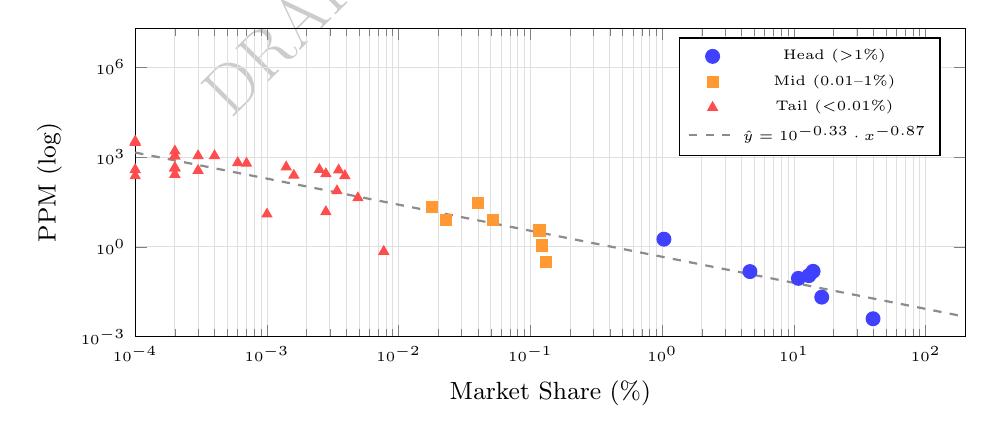
\begin{tikzpicture}
\begin{loglogaxis}[
  width=\columnwidth,
  height=5.5cm,
  xlabel={Market Share (\%)},
  ylabel={PPM (log)},
  xmin=0.0001, xmax=200,
  ymin=0.001, ymax=20000000,
  grid=both,
  grid style={line width=0.3pt, draw=gray!25},
  tick label style={font=\tiny},
  label style={font=\small},
  legend style={font=\tiny, at={(0.97,0.97)}, anchor=north east},
]
\addplot[only marks, mark=*, mark size=2.5pt, color=blue!75]
  coordinates {
    (39.80,0.004)(16.24,0.021)(13.96,0.153)
    (12.97,0.110)(10.80,0.089)(4.63,0.150)(1.03,1.812)};
\addlegendentry{Head ($>$1\%)}
\addplot[only marks, mark=square*, mark size=2pt, color=orange!80]
  coordinates {
    (0.131,0.322)(0.123,1.108)(0.117,3.518)
    (0.052,7.969)(0.040,28.916)(0.023,7.945)(0.018,21.829)};
\addlegendentry{Mid (0.01--1\%)}
\addplot[only marks, mark=triangle*, mark size=2pt, color=red!70]
  coordinates {
    (0.0077,0.703)(0.0049,43.3)(0.0039,238.6)(0.0035,368.0)(0.0034,74.2)
    (0.0028,275.1)(0.0028,14.9)(0.0025,382.5)(0.0016,245.0)
    (0.0014,464.3)(0.0010,12.4)(0.0007,614.5)(0.0006,647.6)
    (0.0004,1106.8)(0.0003,1099.0)(0.0003,355.4)(0.0002,1581.0)
    (0.0002,1081.7)(0.0002,1071.9)(0.0002,418.3)(0.0002,262.5)
    (0.0002,446.6)(0.0001,3354.1)(0.0001,3065.4)(0.0001,378.5)
    (0.0001,235.1)};
\addlegendentry{Tail ($<$0.01\%)}
\addplot[domain=0.0001:200, samples=150, thick, dashed, color=black!45]
  {10^(-0.33) * x^(-0.87)};
\addlegendentry{$\hat{y}=10^{-0.33}\cdot x^{-0.87}$}
\end{loglogaxis}
\end{tikzpicture}
\caption{PPM vs.\ market share (log-log, $n=39$, share~$>0$). Slope $=-0.87$,
$r=-0.938$; relationship holds with alternate PPM normalizations
(slope $=-0.86$, $r=-0.976$ using annual proxy).
Tail CAs (red triangles) carry failure densities $>10^3\times$ the
head (blue circles). CAs with share~$=0$ (including PKIoverheid,
PPM~$>10^7$) are excluded from the regression but represent the
relationship's logical endpoint.}
\label{fig:ppmscatter}
\end{figure}

\section{The Collapse of Root Program Oversight}
\label{sec:oversight}

\subsection{A Shared Capacity Constraint}
\label{sec:coverage}

Figure~\ref{fig:coverage} plots the annual coverage rate for Chrome,
Mozilla, Apple, and Microsoft from 2017 through 2026~Q1. This metric
measures Bugzilla comment engagement specifically---one channel of root
program governance. Governance activity that occurs through direct CA
correspondence, program-specific incident workflows, CCADB surveys, or
in-person meetings is not captured. This scope limitation is particularly
relevant for Chrome from 2022 onward, when the independent Chrome Root
Program launched its own governance infrastructure alongside the
shared Bugzilla channel.

With that caveat established: Chrome and Mozilla each show a distinct
peak followed by a sustained decline. Chrome peaked at 67.8\% in 2019,
Mozilla at 86.2\% in 2017. Both declined into the 7--25\% range where
they remain. The shape and timing differ---Chrome's decline is two years
later and steeper---but the structural cause is the same in both cases:
coverage fell when a dominant individual reduced engagement, and neither
program had distributed the function across a larger team.

Chrome's 2017 (49.6\%) and 2018 (16.7\%) values reflect sparse Bugzilla
activity before the dominant contributor attributed to Chrome via a Gmail
address began engaging at high volume in 2019~Q3; the quarterly figure
(Figure~\ref{fig:quarterly}) shows this as a step-change in mid-2019
rather than a gradual climb. The 2017--2018 low values are real but
reflect a pre-engagement baseline, not a decline from a prior peak.

Chrome's coverage peaked at 67.8\% in 2019 and declined to 22.6\% in 2022,
remaining in the 15--23\% range through 2025. This period coincides with
broader industry disruption---the COVID-19 pandemic affected remote
collaboration and hiring across the security sector in 2020--2021, and
significant technology industry workforce reductions in 2022--2023
constrained staffing across many security teams. The 2024 corpus (236 bugs)
produced 22.5\% coverage, with 2--4 participants engaging approximately
54 unique bugs---a genuine if partial recovery that reflects active
rebuilding of the Chrome program's oversight capacity. The current Chrome
root program team has meaningfully expanded the program's scope and
requirements; the coverage rate reflects the gap between program ambition
and current comment engagement, not a lack of effort. Chrome's 2026~Q1
rate of 9.3\% represents a further decline from 2025's 18.4\%, though
quarterly variation at low coverage levels should be interpreted
cautiously.

Mozilla's decline began earlier, in 2020, when the dominant Mozilla
substantive contributor---responsible for 47\% of all Mozilla governance
comments, active 2017~Q4 through 2020~Q2---departed their Mozilla root
program role. After that departure, Mozilla's coverage stabilized in the
21--26\% range from 2020 through 2023. In 2024, coverage rose to 32.2\%
with the 236-bug corpus---a genuine partial recovery, suggesting the
capacity to rebuild was present. That recovery did not hold: in 2025
coverage fell to 9.9\% (2026~Q1: 6.7\%), with a single
\texttt{@mozilla.com} contributor maintaining activity---40 comments in
2025~Q1, falling to 9, 9, 1 in subsequent quarters. The 2024 uptick
makes the 2025 collapse more striking, not less: the engagement capacity
existed briefly, then did not. Mozilla's program continues to actively
participate in CABF policy work and ballot activity; the coverage rate
captures specifically the Bugzilla comment engagement channel, not program
activity overall.

The combined oversight coverage across all four programs in 2026~Q1 is
lower than at any prior point in the measurement window. Apple is a
meaningful counterpoint: rising from zero to 14.7\% with three active
contributors since 2025~Q4. The ecosystem is not uniformly declining;
new participants are entering as others have reduced their engagement.

\begin{figure}[t]
\centering
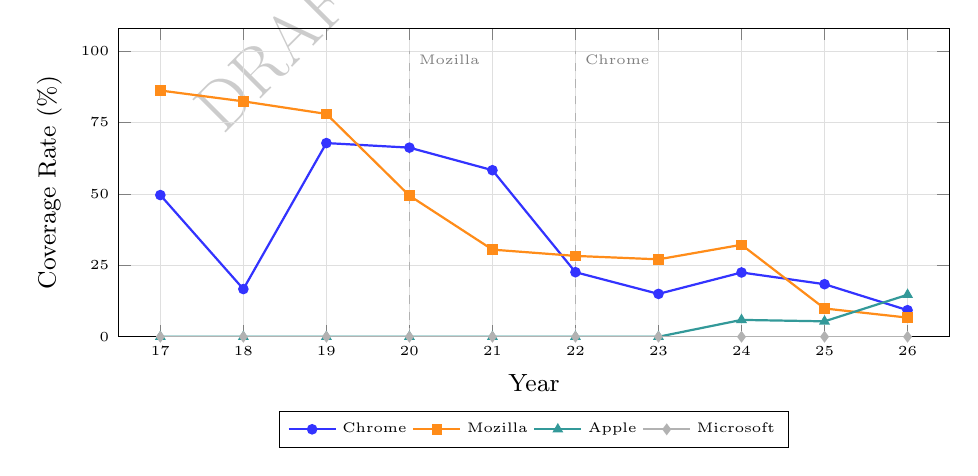
\begin{tikzpicture}
\begin{axis}[
  width=\columnwidth,
  height=5.5cm,
  xlabel={Year},
  ylabel={Coverage Rate (\%)},
  xmin=2016.5, xmax=2026.5,
  ymin=0, ymax=108,
  xtick={2017,2018,2019,2020,2021,2022,2023,2024,2025,2026},
  xticklabels={17,18,19,20,21,22,23,24,25,26},
  ytick={0,25,50,75,100},
  grid=major,
  grid style={line width=0.3pt, draw=gray!25},
  tick label style={font=\tiny},
  label style={font=\small},
  legend style={font=\tiny, at={(0.5,-0.24)}, anchor=north, legend columns=4},
]
% Mozilla dominant contributor departs
\draw[gray!60, dashed] (axis cs:2020,0) -- (axis cs:2020,100)
  node[pos=0.97, right, font=\tiny, color=gray] {Mozilla};
% Chrome dominant contributor departs
\draw[gray!60, dashed] (axis cs:2022,0) -- (axis cs:2022,100)
  node[pos=0.97, right, font=\tiny, color=gray] {Chrome};
\addplot[blue!80, thick, mark=*, mark size=1.5pt] coordinates {
  (2017,49.6)(2018,16.7)(2019,67.8)(2020,66.2)
  (2021,58.3)(2022,22.6)(2023,15.0)(2024,22.5)(2025,18.4)(2026,9.3)};
\addlegendentry{Chrome}
\addplot[orange!90, thick, mark=square*, mark size=1.5pt] coordinates {
  (2017,86.2)(2018,82.4)(2019,78.0)(2020,49.4)
  (2021,30.5)(2022,28.3)(2023,27.1)(2024,32.2)(2025,9.9)(2026,6.7)};
\addlegendentry{Mozilla}
\addplot[teal!80, thick, mark=triangle*, mark size=1.5pt] coordinates {
  (2017,0)(2018,0)(2019,0)(2020,0)(2021,0)
  (2022,0)(2023,0)(2024,5.9)(2025,5.4)(2026,14.7)};
\addlegendentry{Apple}
\addplot[gray!60, thick, mark=diamond*, mark size=1.5pt] coordinates {
  (2017,0)(2018,0)(2019,0)(2020,0)(2021,0)
  (2022,0)(2023,0)(2024,0)(2025,0)(2026,0)};
\addlegendentry{Microsoft}
\end{axis}
\end{tikzpicture}
\caption{Annual Bugzilla oversight coverage rate, 2017--2026~Q1. Both
Chrome and Mozilla show high coverage through 2019--2021, then declining
following reduced engagement by dominant individual contributors (Mozilla
2020~Q2, Chrome 2022~Q2). The Chrome decline coincides with the launch
of an independent Chrome Root Program in September 2022, which shifted
some governance activity to program-specific channels not captured by
this metric. Apple's rising participation is the sole positive trend.
Microsoft's Bugzilla governance coverage is zero throughout.}
\label{fig:coverage}
\end{figure}

\begin{figure}[t]
\centering
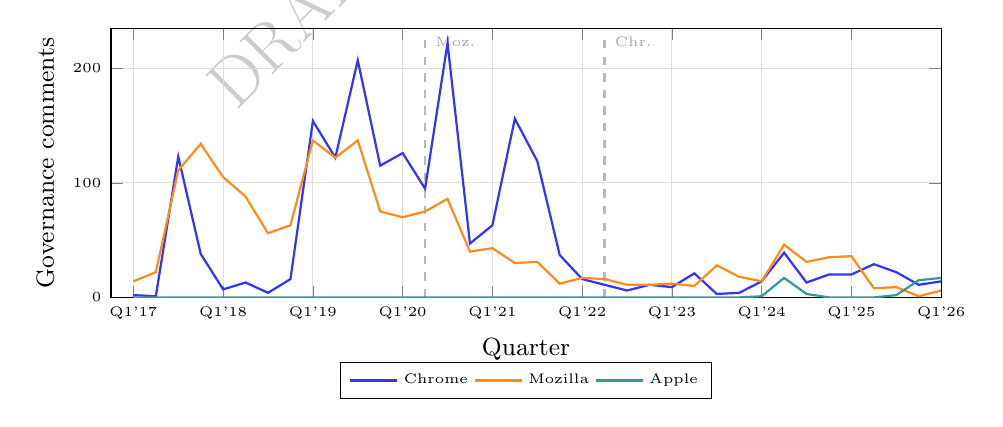
\begin{tikzpicture}
\begin{axis}[
  width=\columnwidth,
  height=5cm,
  xlabel={Quarter},
  ylabel={Governance comments},
  xmin=0, xmax=37,
  ymin=0, ymax=235,
  xtick={1,5,9,13,17,21,25,29,33,37},
  xticklabels={Q1'17,Q1'18,Q1'19,Q1'20,Q1'21,Q1'22,Q1'23,Q1'24,Q1'25,Q1'26},
  tick label style={font=\tiny},
  label style={font=\small},
  grid=major,
  grid style={line width=0.3pt, draw=gray!25},
  legend style={font=\tiny, at={(0.5,-0.24)}, anchor=north, legend columns=3},
]
% Departure markers
\draw[gray!55, dashed, line width=0.8pt]
  (axis cs:14,0) -- (axis cs:14,230)
  node[pos=0.97, right, font=\tiny, color=gray!70] {Moz.};
\draw[gray!55, dashed, line width=0.8pt]
  (axis cs:22,0) -- (axis cs:22,230)
  node[pos=0.97, right, font=\tiny, color=gray!70] {Chr.};
% Chrome quarterly (index 1=2017Q1)
\addplot[blue!80, thick, mark=none] coordinates {
  (1,2)(2,1)(3,123)(4,38)
  (5,7)(6,13)(7,4)(8,16)
  (9,154)(10,122)(11,207)(12,115)
  (13,126)(14,95)(15,222)(16,47)
  (17,63)(18,156)(19,119)(20,37)
  (21,16)(22,11)(23,6)(24,11)
  (25,9)(26,21)(27,3)(28,4)
  (29,14)(30,39)(31,13)(32,20)
  (33,20)(34,29)(35,22)(36,11)
  (37,14)};
\addlegendentry{Chrome}
% Mozilla quarterly
\addplot[orange!90, thick, mark=none] coordinates {
  (1,14)(2,22)(3,111)(4,134)
  (5,105)(6,88)(7,56)(8,63)
  (9,137)(10,122)(11,137)(12,75)
  (13,70)(14,75)(15,86)(16,40)
  (17,43)(18,30)(19,31)(20,12)
  (21,17)(22,16)(23,11)(24,11)
  (25,12)(26,10)(27,28)(28,18)
  (29,14)(30,46)(31,31)(32,35)
  (33,36)(34,8)(35,9)(36,1)
  (37,6)};
\addlegendentry{Mozilla}
% Apple quarterly
\addplot[teal!80, thick, mark=none] coordinates {
  (1,0)(2,0)(3,0)(4,0)
  (5,0)(6,0)(7,0)(8,0)
  (9,0)(10,0)(11,0)(12,0)
  (13,0)(14,0)(15,0)(16,0)
  (17,0)(18,0)(19,0)(20,0)
  (21,0)(22,0)(23,0)(24,0)
  (25,0)(26,0)(27,0)(28,0)
  (29,1)(30,17)(31,3)(32,0)
  (33,0)(34,0)(35,2)(36,15)
  (37,17)};
\addlegendentry{Apple}
\end{axis}
\end{tikzpicture}
\caption{Quarterly governance comment volume by root program, 2017~Q1--2026~Q1.
Chrome (blue) and Mozilla (orange) each show a step-down at their respective
departure events (dashed lines: Mozilla 2020~Q2, Chrome 2022~Q2), two years
apart but structurally identical in shape. Apple (teal) activity begins
only in 2024~Q2. The quarterly granularity makes the two-year offset between
the collapses visible in a way annual coverage rates do not.}
\label{fig:quarterly}
\end{figure}

\subsection{Structural Cause: Key-Person Governance}
\label{sec:keyperson}

The two declines differ in timing and steepness but share a structural
vulnerability: governance quality was concentrated in a small number of
individuals without redundancy.
Figure~\ref{fig:quarterly} shows the quarterly comment volume for all
four programs from 2017 through 2026~Q1; the two step-downs are visible
as structurally similar events separated by two years.

For Chrome, a single contributor attributed to Chrome via a Gmail address
in the Observatory pipeline authored 87\% of all Chrome oversight comments
through 2022~Q2, with 6 unique contributors total. After Q2~2022, Chrome
oversight dropped sharply: from approximately 60 comments per quarter
during 2020--2021 to fewer than 25 per quarter in 2023--2025.

Three structural changes coincide with this period and are important
confounders. First, September 2022 marks the formal launch of the
independent Chrome Root Program---a deliberate strategic decision to allow
Chrome to move faster and more autonomously on trust decisions rather than
continuing to operate primarily through Mozilla's CCADB and Bugzilla
infrastructure. The coverage rate metric measures Bugzilla comment activity
specifically; governance activity that shifted to program-specific channels
(direct CA outreach, the Chrome CCADB annual survey, Chrome's own incident
response workflows) is not captured. The Chrome Root Program's independent
policy has grown substantially more rigorous since 2022, with requirements
on dedicated TLS hierarchies, root term limits, succession planning, and
automation support that exceed the CABF baseline. Second, the 2022--2023
technology industry workforce reductions affected security teams broadly.
Third, the 2023 eIDAS Article~45 debate---in which the EU proposed
legislation that would have compelled browsers to trust government-designated
certificate authorities and restricted the ability to distrust them---raised
genuine legal questions about root program independence that led organizations
to review their governance posture. The provision was ultimately not enacted
in its most aggressive form following coordinated industry opposition, but
the episode surfaced legal and regulatory exposure around distrust decisions
that corporate legal teams continue to assess.

The 2024 partial recovery (22.9\% coverage with 2--4 participants)
represents active rebuilding of the Bugzilla engagement channel alongside
continued development of the program's independent infrastructure. The
March 2025 bulk addition of 110 roots to the Chrome Root Store---visible
in the Observatory's changelog---reflects the program's expanded scope and
ambition. Coverage rate and program scale have moved in opposite directions,
which is itself a finding: the Chrome Root Program has grown more
comprehensive while its public Bugzilla engagement has decreased.

For Mozilla, the dominant contributor accounted for 47\% of all Mozilla
oversight comments, with 9 unique contributors total and the top 3
producing 90\%. Their departure in 2020~Q2 produced a coverage decline
from approximately 55--78\% (2017--2019) to 26--35\% (2020--2021), then
stabilizing in the 22--29\% range through 2024. A second decline in 2025
(9.9\%) corresponds to reduced Bugzilla activity from the single remaining
active \texttt{mozilla.com} contributor. Both Google and Mozilla undertook
significant organizational restructuring in 2023--2024 to redirect
resources toward AI development priorities; the downstream effects on
security infrastructure staffing are not fully visible in public records
but are a plausible contributing factor to the 2025 decline. Mozilla's
program remains active in CABF policy processes; this metric specifically
captures Bugzilla comment engagement.

Apple presents the clearest positive signal. Its coverage rose from zero
to 14.7\% in 2026~Q1---three contributors, all active since 2025~Q4.
The direction is the opposite of Chrome and Mozilla, and the trajectory
suggests a program deliberately building oversight capacity.

The enforcement record provides important context for the coverage rate
numbers. Chrome and Mozilla together initiated the Entrust distrust in
2024---after a 2,644-day documented pattern, the longest runway in the
dataset. Symantec's 2017 distrust involved a CA that at the time held
approximately 30\% of the certificate market; the negotiated transition
and 12-month subscriber migration period it required established the
operational template for large-CA distrust~\cite{amann2017}. Entrust, at roughly 1\%
market share at distrust, required less subscriber migration but had a
substantially longer runway, reflecting the asymmetry between
investigation duration and CA size. Both cases demonstrate that the
enforcement function can act on sufficiently documented patterns. The
coverage rate measures one dimension of the oversight function's health;
the distrust record measures another, and on that dimension the ecosystem
has demonstrated it can act even on commercially significant CAs.

\begin{figure}[t]
\centering
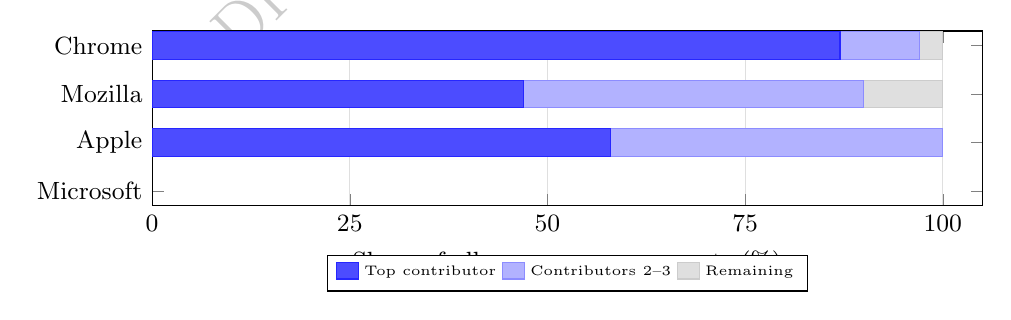
\begin{tikzpicture}
\begin{axis}[
  width=\columnwidth,
  height=3.8cm,
  xbar stacked,
  xlabel={Share of all governance comments (\%)},
  symbolic y coords={Microsoft,Apple,Mozilla,Chrome},
  ytick=data,
  xmin=0, xmax=105,
  xtick={0,25,50,75,100},
  tick label style={font=\small},
  label style={font=\small},
  bar width=10pt,
  xmajorgrids=true,
  ymajorgrids=false,
  grid style={line width=0.3pt, draw=gray!25},
  legend style={font=\tiny, at={(0.5,-0.28)}, anchor=north, legend columns=3},
]
\addplot[fill=blue!70, draw=blue!85] coordinates {
  (87,Chrome)(47,Mozilla)(58,Apple)(0,Microsoft)};
\addlegendentry{Top contributor}
\addplot[fill=blue!30, draw=blue!45] coordinates {
  (10,Chrome)(43,Mozilla)(42,Apple)(0,Microsoft)};
\addlegendentry{Contributors 2--3}
\addplot[fill=gray!25, draw=gray!40] coordinates {
  (3,Chrome)(10,Mozilla)(0,Apple)(0,Microsoft)};
\addlegendentry{Remaining}
\end{axis}
\end{tikzpicture}
\caption{Governance comment concentration by root program. Chrome's top
contributor accounts for 87\% of all oversight comments; the top 3
produce 97\%. Mozilla is less concentrated but the top contributor
still holds 47\%. Apple, newly active, mirrors Chrome's early
concentration pattern. Microsoft has zero governance comments and
therefore no contributors to measure.}
\label{fig:concentration}
\end{figure}

\subsection{The Governance Incident Surge and Its Interpretation}
\label{sec:govsurge}

Figure~\ref{fig:incmix} shows the shifting composition of annual incidents.
Through 2024, governance failures (audit qualifications, CPS violations,
disclosure failures) accounted for 17--40\% of filings annually. In 2025,
governance reached 60\% (129 of 214 incidents); in 2026~Q1, 55\%
(36 of 66).

This requires explanation. Reduced oversight should, if anything, reduce
reported governance failures---if no one is pressing for root cause,
fewer process failures surface. The data shows the opposite. Two mechanisms
explain the divergence.

First, audit-initiated discovery rose sharply: from under 5\% annually
through 2024 to 24\% in 2025 (52 incidents). Auditors have structured
incentives to surface process failures that continuous oversight previously
handled informally. As real-time scrutiny declined, the annual audit became
a slower but more systematic backstop.

Second, the MPIC requirement (multi-perspective issuance corroboration)
took effect in 2025, generating a wave of CPS update obligations many of
which appear as governance incidents. The absolute misissuance count fell
in 2025 (34 vs.\ 80 in 2024) while governance rose. The surge is a
category shift, not an operational collapse---though the audit discovery
data suggests governance failures were previously underreported.

\begin{figure}[t]
\centering
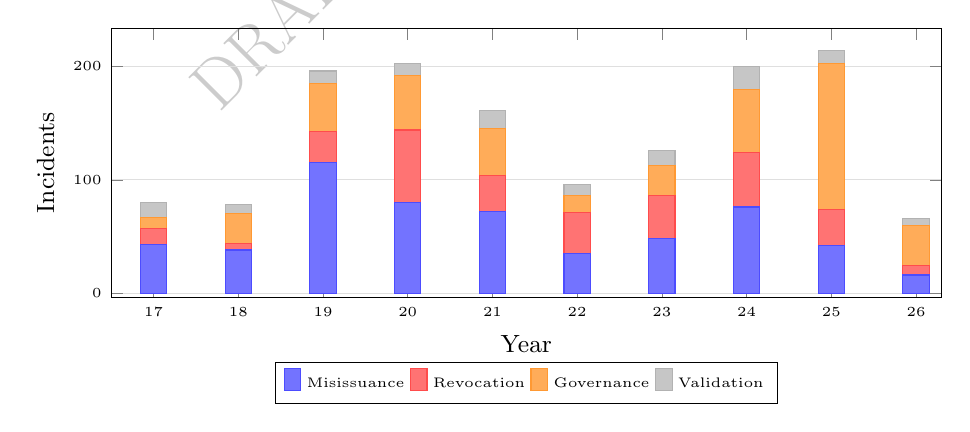
\begin{tikzpicture}
\begin{axis}[
  width=\columnwidth,
  height=5cm,
  ybar stacked,
  xlabel={Year},
  ylabel={Incidents},
  xmin=2016.5, xmax=2026.3,
  xtick={2017,2018,2019,2020,2021,2022,2023,2024,2025,2026},
  xticklabels={17,18,19,20,21,22,23,24,25,26},
  bar width=9.5pt,
  ymajorgrids=true,
  grid style={line width=0.3pt, draw=gray!25},
  tick label style={font=\tiny},
  label style={font=\small},
  legend style={font=\tiny, at={(0.5,-0.24)}, anchor=north, legend columns=4},
]
\addplot[fill=blue!55, draw=blue!70] coordinates {
  (2017,43)(2018,38)(2019,115)(2020,80)(2021,72)
  (2022,35)(2023,48)(2024,76)(2025,42)(2026,16)};
\addlegendentry{Misissuance}
\addplot[fill=red!55, draw=red!70] coordinates {
  (2017,14)(2018,6)(2019,28)(2020,64)(2021,32)
  (2022,36)(2023,38)(2024,48)(2025,32)(2026,8)};
\addlegendentry{Revocation}
\addplot[fill=orange!65, draw=orange!80] coordinates {
  (2017,10)(2018,26)(2019,42)(2020,48)(2021,41)
  (2022,15)(2023,27)(2024,56)(2025,129)(2026,36)};
\addlegendentry{Governance}
\addplot[fill=gray!45, draw=gray!60] coordinates {
  (2017,13)(2018,8)(2019,11)(2020,11)(2021,16)
  (2022,10)(2023,13)(2024,20)(2025,11)(2026,6)};
\addlegendentry{Validation}
\end{axis}
\end{tikzpicture}
\caption{Annual incident volume by classification, 2017--2026 (2026 = Q1
only). Governance incidents (orange) surge to 60\% in 2025, driven by
audit-initiated discovery and MPIC-related CPS obligations---not by
worsening CA operations. Misissuance actually declined in 2025.}
\label{fig:incmix}
\end{figure}

\subsection{Discovery Channel Analysis: CAs Are Monitoring Themselves}
\label{sec:discovery}

Table~\ref{tab:discovery} shows the discovery channel distribution
for the 1,505-bug corpus. The most significant finding is a structural
shift in who detects compliance failures. CA self-filing---incidents
the CA's own monitoring and linting infrastructure identified and
reported without external prompting---accounts for 21.8\% of all-time
bugs and has surged to 46.1\% in 2025 and 43.2\% in 2026~Q1. Root
programs initiate only 4.1\% all-time. Unknown---bugs where no
first-comment text was available for classification, typically because
the scrape captured the bug before any comment was posted---accounts
for 29.4\%.

The Unknown category warrants substantive treatment. Its annual share
ranges from roughly 9\% to 44\% across the measurement window, with
the elevated values in earlier years reflecting sparser initial
comment availability; recent years are more complete: 2025 (11.4\%),
2026~Q1 (25.7\%). Unknown does not skew toward any particular program
or CA type---it is a uniform pipeline artifact of scraping lag, not a
classification ambiguity. Under proportional redistribution of Unknown
across the classified channels, CA self-filing rises from 21.8\% to
30.9\%, Community/CT/linting from 17.3\% to 24.6\%, and Root program
from 4.1\% to 5.8\%. The central finding---CA self-filing is now the
dominant channel, with CT linting well ahead of root programs in
all-time absolute volume---is invariant to any redistribution
assumption.

The all-time CT/linting share of 17.3\% reflects its substantial role
in the 2017--2024 period, when it initiated between 15\% and 48\% of
annual incidents. A naive reading of the Bugzilla record---counting
bare occurrences of browser vendor names in CA-authored compliance
text---would suggest root programs initiate the majority of bugs. The
attribution methodology in Section~\ref{sec:attribution} shows that
pattern is an artifact of CA operators referencing program names in
their own disclosures. The measured root program initiation rate of
4.1\% all-time establishes that what root programs have historically
provided is \textit{investigative pressure after detection}, not
primary detection.

The 2025--2026 surge in CA self-filing requires careful interpretation.
The absolute count rose from 23 in 2023 to 82 in 2024 and 101 in
2025. The incident category driving it matters: governance incidents
surged to 60\% of the 2025 corpus, and the MPIC requirement
(multi-perspective issuance corroboration) generated a wave of CPS
update obligations that took effect that year. These are precisely the
incident type that CT linting cannot surface---they are failures of
process description and documentation, not failures visible in
certificate bytes. Well-resourced CAs with internal compliance teams
identified and filed their own CPS deficiencies before auditors or
external parties found them. The self-filing surge is therefore not a
generic improvement in CA monitoring culture; it is a specific response
to a specific new obligation by the CAs with the institutional capacity
to respond proactively. ISRG (Let's Encrypt) has historically filed
50\% of its own incidents~\cite{aas2019}; the 2025 surge suggests
other large CAs are building similar pre-filing discipline for the
governance incident category in particular. The rise in CA self-filing
occurring simultaneously with declining root program coverage suggests
the ecosystem is beginning to internalize the monitoring function that
external oversight capacity can no longer reliably provide---but the
internalization is concentrated in the CAs that need it least.

\textbf{The CT detection infrastructure and its dependencies.}
The community/CT/linting channel that accounts for 17.3\% of all-time
incident bugs rests on a toolchain assembled over a decade through
largely volunteer and single-organization effort. CT itself was
standardized in RFC~6962~\cite{laurie2014} and mandated by Chrome from
January 2018; Google's Trillian log backend (2016) provides the
server-side infrastructure operated by Google, Cloudflare, DigiCert,
and others. The linting layer---zlint (2016, the zmap research group
at University of Michigan, now maintained by a distributed community
of Mozilla, ISRG, and Google contributors without dedicated funding)
and crt.sh (2015, operated by Sectigo through a single
engineer)---converts CT log data into actionable compliance
signals~\cite{sun2024}. This toolchain has no formal governance, no
minimum staffing requirements, and no explicit funding commitments
from the ecosystem that depends on it.

A critical structural limitation bounds what this toolchain can detect.
CT linting reads certificate contents---key sizes, field encodings,
serial entropy, profile conformance---and surfaces violations visible
in the bytes. It cannot detect whether a CA's CPS accurately describes
its actual validation procedures, whether an incident response plan is
credible, whether an audit qualification was adequately disclosed, or
whether a CA's root cause analysis reflects genuine process change.
These governance failures---which constitute 60\% of all incidents in
2025---are invisible to any tool that examines certificates alone.
This is precisely why the coverage rate metric matters: it measures
the human investigation layer that reaches categories of failure no
automated tool can see.

The parallel to aviation safety reporting is instructive. Aircraft
accident investigation agencies collect incident reports not merely to
count events, but to classify them, identify systemic patterns, and
route findings to the actors with authority to change underlying
conditions. A near-miss that surfaces a procedural gap in a checklist
is more valuable than ten incidents caused by the same equipment
failure that linters could have caught. The WebPKI's governance
commentary on Bugzilla incidents serves the same function: it assesses
whether a CA's response reflects genuine process improvement or managed
disclosure, and routes that assessment toward the distrust decision
when warranted. The 2024 Entrust action was not triggered by a linter
finding a misissued certificate; it was triggered by years of
investigative commentary concluding that the pattern of compliance
posture was irremediable. Automated detection and human investigation
are complements, not substitutes.

Two structural observations follow from the discovery data. First, the
absolute volume of CT/community initiated bugs has declined in
2025--2026 (16 and 1 respectively) as the incident corpus has grown
into governance categories that certificate-content linters cannot
reach; the CT toolchain remains load-bearing for what it can see, but
the most consequential incident categories now require human or
internal audit detection. Second, Chrome is the primary steward of the
next-generation CT infrastructure: the tiled log specification
(Sunlight, 2023) and the active IETF Merkle Tree Certificates draft
(2026) represent deliberate investment toward a more scalable
successor. This is a positive development, but it concentrates the
evolutionary trajectory of the detection layer in one organization's
product and standards priorities.

\begin{table}[t]
\centering
\footnotesize
\caption{Discovery channel distribution across 1,505 non-distrusted
Bugzilla compliance bugs (2014--2026). The corpus excludes bugs filed
by CAs subsequently distrusted by all programs; the 77-bug gap from
the 1,428 incident count reflects sub-operator naming variants
(e.g., ``DigiCert / ABB'') normalized into parent CA counts in the
incident analysis but retained here. CA self-filing is the dominant
channel in 2025--2026, driven by growing internal monitoring investment.
The audit channel's rise in 2025 (23.7\%) partially compensates for
declining real-time root program oversight.}
\label{tab:discovery}
\begin{tabularx}{\columnwidth}{@{}Xrrr@{}}
\toprule
Channel & All-time & 2025 & 2026 Q1 \\
\midrule
CA self-filed            & 21.8\% & 46.1\% & 43.2\% \\
Unknown                  & 29.4\% & 11.4\% & 25.7\% \\
External researcher      & 19.5\% &  5.9\% &  9.5\% \\
Community / CT / linting & 17.3\% &  7.3\% &  1.4\% \\
Audit                    &  7.8\% & 23.7\% & 13.5\% \\
Root program             &  4.1\% &  5.5\% &  6.8\% \\
\bottomrule
\end{tabularx}
\end{table}

\begin{figure}[t]
\centering
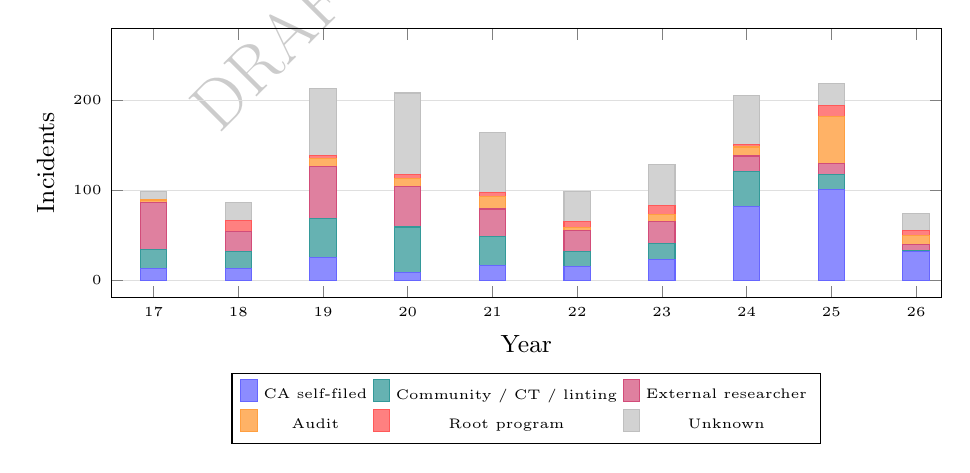
\begin{tikzpicture}
\begin{axis}[
  width=\columnwidth,
  height=5cm,
  ybar stacked,
  xlabel={Year},
  ylabel={Incidents},
  xmin=2016.5, xmax=2026.3,
  xtick={2017,2018,2019,2020,2021,2022,2023,2024,2025,2026},
  xticklabels={17,18,19,20,21,22,23,24,25,26},
  bar width=9.5pt,
  ymajorgrids=true,
  grid style={line width=0.3pt, draw=gray!25},
  tick label style={font=\tiny},
  label style={font=\small},
  legend style={font=\tiny, at={(0.5,-0.28)}, anchor=north, legend columns=3},
  ymax=280,
]
\addplot[fill=blue!45, draw=blue!60] coordinates {
  (2017,13)(2018,13)(2019,25)(2020,8)(2021,16)
  (2022,15)(2023,23)(2024,82)(2025,101)(2026,32)};
\addlegendentry{CA self-filed}
\addplot[fill=teal!60, draw=teal!80] coordinates {
  (2017,21)(2018,19)(2019,43)(2020,51)(2021,32)
  (2022,17)(2023,18)(2024,39)(2025,16)(2026,1)};
\addlegendentry{Community / CT / linting}
\addplot[fill=purple!50, draw=purple!70] coordinates {
  (2017,52)(2018,22)(2019,58)(2020,45)(2021,31)
  (2022,23)(2023,24)(2024,17)(2025,13)(2026,7)};
\addlegendentry{External researcher}
\addplot[fill=orange!60, draw=orange!75] coordinates {
  (2017,3)(2018,0)(2019,9)(2020,9)(2021,14)
  (2022,3)(2023,8)(2024,10)(2025,52)(2026,10)};
\addlegendentry{Audit}
\addplot[fill=red!50, draw=red!65] coordinates {
  (2017,1)(2018,12)(2019,4)(2020,4)(2021,4)
  (2022,7)(2023,10)(2024,3)(2025,12)(2026,5)};
\addlegendentry{Root program}
\addplot[fill=gray!35, draw=gray!50] coordinates {
  (2017,9)(2018,20)(2019,74)(2020,91)(2021,67)
  (2022,34)(2023,46)(2024,54)(2025,25)(2026,19)};
\addlegendentry{Unknown}
\end{axis}
\end{tikzpicture}
\caption{Incident discovery channel by year, 2017--2026. CA self-filing
(blue) has become the dominant channel in 2025--2026, rising from a
historical baseline of 8--16\% to 46.1\% in 2025 and 43.2\% in
2026~Q1. The 2025 audit spike (orange) reflects structured auditor
incentives partially compensating for declining root program
engagement (red). Community/CT/linting (teal) remains significant
all-time but has declined as governance incidents---invisible to
certificate-content linters---now dominate the corpus.}
\label{fig:discovery}
\end{figure}

\subsection{The Comprehension Gap}
\label{sec:participation}

The discovery channel data shows that incident detection is being handled
by CAs, auditors, and automated tools---not root program staff. The
standards side of the governance process shows a different gap. Of 56 CA/B
Forum member organizations, \textbf{35 (62.5\%)} have contributed zero
engagement to the public compliance record: no Bugzilla comments on other
CAs' incidents, no ballot proposals or endorsements, no proactive incident
filings. Earlier measurements of this corpus recorded non-participation rates
above 80\%, when the denominator included all 62 organizations in the
CCADB with some CABF affiliation. The current 62.5\% uses the stricter
denominator of formal CABF CA member organizations (56), and reflects
a cohort of newer programs that have built some participation capacity
since that earlier count---but the governance structure underneath
has not changed.

The concern is not primarily that these organizations should be contributing
more to governance. The ecosystem would not necessarily benefit from 35
additional organizations engaging at variable quality in standards
discussions or linting toolchains; experience with open-source compliance
tooling suggests that low-quality engagement from organizations without
the engineering depth to contribute meaningfully can be actively
counterproductive, consuming reviewer capacity without improving outcomes.
The concern is epistemic: for these 35
organizations, there is no public signal that they are tracking changes to
the requirements they are bound by. When a ballot modifies certificate
profile requirements or a Bugzilla thread establishes a new enforcement
interpretation, the only evidence that these CAs are aware of the
change---let alone implementing it---arrives at the next annual audit,
which prior work in this series has established catches only 29.2\% of
in-period incidents~\cite{p2}. Non-participation is not primarily a
contribution gap. It is an observability gap: the governance system has no
mechanism for distinguishing a CA that silently tracks every requirement
change from one that has no idea what changed last quarter.

CA/B Forum membership carries voting rights on the Baseline Requirements.
These 35 organizations vote on rules they show no evidence of tracking.
This is not a democratic legitimacy concern; it is an information asymmetry
in which the organizations writing requirements have no mechanism to verify
that the organizations bound by them have read them.

The comprehension gap is two-sided. On one side, 62.5\% of member
organizations show no observable engagement with requirements evolution.
On the other, the requirements themselves are being written by a
concentrated set of contributors. Among non-root-program contributors,
one individual has personally engaged 109 bugs and filed 60 proactive
incident reports---more governance contribution than all but two member
organizations. The WebPKI's collective governance capacity is not merely
thin at the institutional level; it is thin enough that a single private
individual's voluntary participation is load-bearing. The ballot process
mirrors this pattern: one individual has personally proposed 36 of the
Forum's ballots, with the top five individual proposers accounting for
the majority of all substantive policy submissions across four working
groups. Three of the top five ballot proposers are employed by a single
CA operator (DigiCert), meaning the organization with the largest all-time
incident count (171) and the worst audit transparency gap (98.2\%) is also
the dominant author of the rules every CA must follow. The process produces
rules without evidence that they are understood by those they bind,
authored disproportionately by an organization whose own compliance record
suggests the rules have not prevented its own recurring failures.

\section{The Microsoft Root Store as a Governance Enclave}
\label{sec:microsoft}

The coverage rate decline documented in Section~\ref{sec:oversight} raises
a question: what does sustained zero oversight coverage look like in
practice? The Microsoft Root Store provides the clearest existing answer.

Microsoft's governance posture requires precise description. Its 310-root,
84-owner trust store is the largest of the four major programs by both
counts, contains 142 roots exclusive to it, and has produced
\textbf{zero} governance oversight comments on other CAs' compliance
incidents across the entire 2014--2026 measurement window.

This statement requires the definitional precision the pipeline provides.
Microsoft PKI Services is a publicly trusted CA (rank 6, 4.63\% market
share, 47 incidents in the corpus). When its \texttt{@microsoft.com} staff
respond to their own incident bugs, those comments are CA-operator activity.
The pipeline explicitly classifies self-incident comments separately from
governance comments~\cite{github-code}. Of 494 total Microsoft Bugzilla
comments, 493 are self-incident responses and 1 is classified as
administrative process. After that separation, the governance comment count
is zero. The 494 total comments and the zero governance comments are not
in tension---they describe different activities.

The consequence of this posture is structural. Microsoft's 142 exclusive
roots have no peer-program reference for compliance comparison and face no
external oversight pressure from Chrome, Mozilla, or Apple. Those CAs are
also not visible to the community of researchers who monitor Mozilla
Bugzilla, because CAs exclusive to Microsoft do not file there.

Microsoft's enforcement record further characterizes its posture. Of 15
distrust events where peer programs acted between 2011 and 2024, Microsoft
acted on 11. It has never initiated a distrust action. It chose not to
follow peers in four cases: India CCA (2014), Certinomis (2019),
Camerfirma (2021), and Visa (2022). All four remain in the Microsoft store
today. Microsoft's browser-side market share is effectively zero (Edge uses
Chrome's root store), but its store matters for Windows enterprise TLS,
S/MIME, and code signing---contexts not captured by browser share metrics.
For CAs exclusive to the Microsoft store, the structural absence of
cross-program oversight means internal self-assessment is the only
available monitoring mechanism: external investigative pressure from
peer programs does not reach them.

The four trust divergences are summarized in Table~\ref{tab:divergence}.

\begin{table}[t]
\centering
\footnotesize
\caption{CAs distrusted by Chrome, Mozilla, and Apple but still in the
Microsoft store as of March 2026.}
\label{tab:divergence}
\begin{tabularx}{\columnwidth}{@{}lllX@{}}
\toprule
CA & Year & Posture & Reason \\
\midrule
India CCA & 2014 & Negligent & Unauthorized cert issuance; govt CA \\
Certinomis & 2019 & Negligent & Pattern of BR violations; non-responsive \\
Camerfirma & 2021 & Negligent & Multi-year BR pattern; delayed revocation \\
Visa        & 2022 & Negligent & BR violations; non-responsive \\
\bottomrule
\end{tabularx}
\end{table}

\section{Distrust Patterns and Runway}
\label{sec:distrust}

The oversight capacity documented in Section~\ref{sec:oversight} feeds a
specific downstream process: the accumulation of public evidence sufficient
for root programs to act. The distrust record establishes how long that
process takes and what fraction of it depends on the Bugzilla channel
whose coverage is declining.

Sixteen CA distrust events occurred between 2011 and 2024.
Table~\ref{tab:runway} shows the ten events with measurable runways---time
from the first public Bugzilla incident to the distrust effective date.
The distribution is:
\begin{itemize}[noitemsep, topsep=2pt]
\item Mean runway: 1,280 days (3.5 years)
\item Median runway: 1,185 days (3.3 years)
\item 7 of 10 exceeded 1,000 days; maximum was 2,644 days (Entrust); 73\% of events followed a response-driven pathway rather than a single catastrophic trigger
\end{itemize}

\begin{table}[t]
\centering
\footnotesize
\caption{Distrust events with measurable runway (days from first public
incident to distrust effective date). Posture codes: A=Argumentative,
N=Negligent, I=Incompetent, W=Willful.}
\label{tab:runway}
\begin{tabularx}{\columnwidth}{@{}Xrll@{}}
\toprule
CA & Days & P & Detection \\
\midrule
Entrust (2024)         & 2,644 & A & Root program \\
e-Tugra (2023)         & 1,930 & I & Researcher \\
Visa (2022)            & 1,750 & N & Root program \\
Camerfirma (2021)      & 1,529 & N & Root program \\
TrustCor (2022)        & 1,185 & N & Journalism \\
Ecommerce Mon.\ (2024) & 1,085 & I & Root program \\
PROCERT (2020)         & 1,020 & I & Root program \\
Certinomis (2019)      &   668 & N & Root program \\
Symantec (2017)        &   620 & A & CT + researcher \\
TurkTrust (2018)       &   372 & N & Root program \\
\bottomrule
\end{tabularx}
\end{table}

The runway is not a property of violation severity. Entrust (2,644 days)
and Certinomis (668 days) both exhibited patterns of accumulated BR
violations. Shorter runways correlate with external researcher discovery
(e-Tugra: researcher found default credentials) or catastrophic single
events involving active harm. The modal path to distrust is 2--5 years
of documented failures accumulating without resolution.

The posture distribution across all 16 events: Negligent 7 (43.8\%),
Willful 3 (18.8\%), Incompetent 3 (18.8\%), Argumentative 2 (12.5\%),
Accidental 1 (6.3\%). The single most consistent finding across all 16
events: \textbf{no CA was distrusted for a single well-handled incident}.
Distrust is always the outcome of an institutional pattern. The governance
model can act decisively---but only after years of accumulated evidence
have made the pattern unmistakable. The question is whether the oversight
capacity to assemble that evidence still exists.

\section{Cryptographic and Jurisdictional Risk}
\label{sec:crypto}

The governance fragilities documented above interact with two additional
risk dimensions that the oversight model must also cover but that receive
minimal systematic attention in the Bugzilla compliance process.

\textbf{Cryptographic posture.} Of the 317 root certificates belonging
to CA owners with active certificate issuance, 43
(13.6\%) carry SHA-1 signatures and one carries an RSA-1024 key
(Government of Spain, FNMT). SHA-1 root self-signatures carry limited
chain-building risk by definition, but signal generation era and create
audit complexity. The RSA-1024 root is more concrete: a 1024-bit key
falls below every major standards body's minimum for all certificate
types. It remains in the Microsoft store.

\textbf{Jurisdictional compellability.} We classify jurisdictions on
three axes: purpose-built key seizure authority, purpose-built compelled
issuance authority, and statutory secrecy preventing disclosure to
auditors. Four jurisdictions have purpose-built authority on all three
axes: China, UK, Australia, Russia. The critical combination is compelled
issuance $+$ secrecy: a CA can be forced to issue fraudulent certificates
and simultaneously prohibited from disclosing the compulsion to root
programs or auditors.

The volumetric exposure is dominated by a single data point: Sectigo,
UK-headquartered, with 10.6\% global market share and 137.2 million
active certificates, operates under RIPA~2000 Part~III and the
Investigatory Powers Act 2016. The UK's Technical Capability Notices
can require operators to remove electronic protection on communications
with a gag order preventing disclosure to root programs. China contributes
336,790 active certificates across eight CA entities; Russia has no
currently trusted CA entities. The 10.6\% ``high-risk'' exposure figure
is almost entirely Sectigo/UK, not China---a distinction that matters
for calibrating the actual threat model.

\section{The 47-Day Transition}
\label{sec:validity}

The preceding sections document a governance apparatus at historically low
capacity. The 47-day validity transition is about to increase the load on
that apparatus substantially.

Certificate maximum validity is reducing in three stages: 200 days
(March 2026, now in effect), 100 days (March 2027), 47 days (March 2029).
We measure CA readiness using the usage period metric: $365 /
(\text{all-time certs} / \text{unexpired certs})$, which captures actual
subscriber replacement behavior rather than the validity period printed
on certificates. A CA issuing 90-day certificates whose subscribers
auto-renew at 60 days has a 22-day usage period and is compliant through
2029; a CA whose subscribers renew at 145 days is not.

Table~\ref{tab:brready} summarizes the readiness landscape.

\begin{table}[t]
\centering
\footnotesize
\caption{BR validity readiness by usage period tier (March 2026).
Cert \% is share of all 1.29B active certificates. The 67.2\% already
automation-ready reflects ISRG (40.1\%), GTS (16.2\%), and Sectigo (10.8\%)
as the dominant contributors.}
\label{tab:brready}
\begin{tabularx}{\columnwidth}{@{}lrrl@{}}
\toprule
Tier & CAs & Certs & Status \\
\midrule
$<$ 47d (automation-ready) & 12 & 67.2\% & Compliant through 2029 \\
47--100d (middle band)     & 21 & 18.7\% & Compliant through 2027 \\
100--200d (100d threshold) &  6 & 14.0\% & Breach March 2027 \\
$>$ 200d (current breach)  &  4 &  0.1\% & Breach today \\
\bottomrule
\end{tabularx}
\end{table}

The four CAs already above 200 days---OISTE (365d), HARICA (340d), NAVER
(309d), TrustAsia (287d)---collectively represent 0.1\% of certificates.
Their subscribers have not established the automation needed for the
threshold now in effect.

The March 2027 100-day threshold is the critical policy horizon. The six
CAs in the 100--200d band represent 14.0\% of all active certificates.
The two largest are GoDaddy (145d, 12.97\% share, $\approx$167M active
certificates) and IdenTrust (130d, 1.03\% share, $\approx$13M certificates
spanning federal PKI, healthcare, and code signing).

The failure modes differ by subscriber profile. GoDaddy's book is
predominantly SMB hosting customers: organizations without DevOps
pipelines, running manual renewal workflows, often on annual cycles.
Their path to the 100-day threshold requires not just ACME automation
but organizational behavior change across a subscriber base with no
history of certificate lifecycle tooling. The dominant risk is expiry
outages when the deadline passes before that change occurs. IdenTrust's
federal and healthcare subscribers face a different constraint: procurement
cycles, change-control requirements, and security authorization processes
that operate on timelines incompatible with automated certificate renewal.
Their risk is equally expiry-driven, with the additional complication that
some certificate uses---S/MIME identity binding, code signing---do not
map cleanly onto ACME's domain-validation model.

GoDaddy subscribers must reduce their mean renewal period from 145 to
under 100 days---a 31.0\% reduction---within 12 months of this writing.
IdenTrust requires a 23.1\% reduction on the same timeline. For the
remaining six CAs in the band, the volumes are small but the pattern
holds: all serve subscriber segments where automation is not yet the
default. The secondary failure mode applies to any CA that attempts to
close the gap by deploying automation rapidly: incorrect ACME
implementations, validation errors under short renewal windows, and
encoding mistakes in high-velocity issuance all generate misissuance,
which arrives into the oversight apparatus at its lowest measured
capacity.

The governance implication is direct. That misissuance arrives into
an oversight apparatus at its lowest measured capacity across the
entire 12-year record. We call this the \textit{velocity-oversight
scissor}: issuance velocity is being driven up by policy while
oversight capacity has declined to its floor. The crossing is not
projected---it is occurring now. When the first wave of subscribers
misses the March~2027 deadline and generates misissuance, the oversight
apparatus that would normally route findings toward enforcement is at
its lowest measured engagement in twelve years. Both pressures peak
simultaneously.

\section{Discussion}
\label{sec:discuss}

\subsection{Why Oversight Capacity Is Fragile}

The multi-program architecture is genuinely resilient at the enforcement
level. Chrome, Mozilla, Apple, and Microsoft each maintain independent root
stores and can act unilaterally on distrust; organizational rot in one
program does not propagate to the others. But that resilience does not
extend to the oversight level. No root program faces consequences for
reducing Bugzilla engagement to zero. There is no minimum coverage
threshold, no staffing standard, and no mechanism that redistributes the
oversight function when one program withdraws. Non-participation is
costless. The Microsoft store demonstrates the endpoint: 142 exclusive
roots, zero governance comments across twelve years, and 34 of 36
exclusive CA owners with zero Bugzilla incident history. For those CAs,
whether the absence of incidents reflects genuine compliance or simply the
absence of anyone looking is, by construction, unknowable from public data.

The WebPKI's governance architecture formalized CA obligations in minute
detail while leaving root program obligations entirely informal. There
is no document specifying what fraction of open incidents a root program
must engage with, what constitutes an adequate response, or how staffing
of the oversight function should be maintained. This is not a design
failure in the ordinary sense---the informal model emerged because root
programs are voluntary, and formalizing obligations for organizations
that participate voluntarily is genuinely difficult.

The consequence is predictable from basic public goods theory. CAs bear
the cost of compliance; root programs bear the cost of oversight. The
benefits of a well-governed ecosystem are diffuse while the costs are
concentrated on the root program engineers who do the work. Individual
contributors internalize these costs through professional commitment.
The governance model is stable while those individuals remain engaged,
and fragile when they do not. Two additional forces documented in
Section~\ref{sec:keyperson} compound this: Chrome's 2022 independent
program launch shifted substantive engagement to channels outside
Bugzilla's visibility, and the 2023 eIDAS Article~45 episode introduced
legal scrutiny around distrust decisions that has no prior precedent.
Neither is captured in the coverage rate metric; both are real constraints
on program behavior.

\subsection{From Detection to Comprehension}
Section~\ref{sec:discovery} establishes that CA self-filing now accounts
for 46.1\% of incidents in 2025 and 43.2\% in 2026~Q1, while root program
staff initiate only 4.1\% all-time. The detection function is being
substantially internalized by CAs themselves---a structural adaptation
occurring simultaneously with the decline in external oversight. The gap
that remains is investigative: internal CA monitoring surfaces encoding
errors and profile violations, but the root program assessment of whether
a CA's response reflects genuine process change, and the escalation to
distrust when it does not, depends on external human reviewers at
historically low capacity.

The self-detection data sharpens the point. Across 1,428 incidents, 21.8\%
all-time were filed by the CA's own staff, rising to 46.1\% in 2025.
ISRG (Let's Encrypt)~\cite{aas2019} files 50\% of its own incidents---a rate
reflecting investment in pre-issuance linting and continuous CT monitoring.
Other large CAs appear to be building similar internal monitoring capacity,
which is a genuine positive signal. The 47-day validity transition will
require the automation infrastructure that makes ISRG's self-detection
rate possible; CAs that have not built it will generate misissuance at
higher velocity with less internal ability to detect it.

But detection is not comprehension, and comprehension is not remediation.
The comprehension gap documented in Section~\ref{sec:participation}
identifies a distinct failure mode: 62.5\% of CABF member organizations
show no observable engagement with the requirements they are bound by.
A CA that detects its own encoding errors but shows no evidence of
tracking requirement changes is solving a different problem than the one
the governance model needs solved. The detection transition is real and
positive; the question is whether it extends to the deeper layers of
the accountability loop.

The fragility this paper documents has a structural cause: the governance
model has no machine-readable record of its own state. Coverage rates,
key-person concentration, discovery channel composition, and CA compliance
trajectories were not measured until the Observatory was built. The
Mozilla dominant contributor departure and its consequences would have been
visible in quarterly data within two quarters of the event---but no
instrument existed to generate that data, and nobody was watching.

This paper is itself a demonstration that continuous automated governance
monitoring is feasible. The same transformation CT brought to certificate
issuance---converting an opaque, episodic process into a continuous,
measurable one---can be applied to the governance layer. CT did not replace
the humans who respond to misissuance; it made misissuance visible enough
that accountability became possible. The same logic applies to oversight.

Three levels of automated monitoring address three distinct fragilities.

At the \textit{detection level}, a meaningful transition is underway:
CA self-filing has reached 46.1\% of incidents in 2025 and CT linting
accounts for 17.3\% all-time, together representing the large majority
of all detected failures without root program initiation. The remaining
gap is routing: neither internal CA monitoring nor certificate-content
linters provide investigators with cross-CA pattern context, open
obligation tracking, or escalation prioritization. Those functions
still require human root program staff.

At the \textit{comprehension level}, the governance system currently has
no mechanism for verifying that CAs track requirement changes between
annual audits. Continuous evaluation---whether through structured
self-assessment, demonstrated engagement with requirement evolution, or
automated posture measurement---would close the observability gap that
makes the 62.5\% non-engagement figure concerning rather than merely
notable.

At the \textit{accountability level}, continuous public measurement creates
pressure without new policy instruments. No root program currently publishes
a coverage rate. No CA can query which of its open Bugzilla bugs has received
a substantive response this quarter. Making these numbers public---as the
Observatory now does---makes sustained inaction visible to the community
and, eventually, to regulators.

At the \textit{institutional resilience level}, structured data dissolves
key-person fragility. When institutional knowledge about CA compliance
histories, open obligations, and recurring patterns lives in one person's
head, the institution loses it when that person leaves. When it lives in
a continuously updated, publicly queryable dataset, it transfers. The
Observatory is a prototype of that institutional memory; the governance
model's fragility is partly a consequence of never having built it before.

The limits of this approach are real. Automated monitoring cannot determine
whether a root cause analysis is credible, whether a remediation commitment
is adequate, or whether a pattern warrants distrust. Those judgments require
domain expertise. What automation provides is that the humans exercising that
judgment are examining the right cases at the right time, rather than
discovering a six-year coverage rate collapse in retrospect.

\subsection{Structural Remedies}
Three policy changes would materially improve the governance model.

Root programs should formalize the oversight function with minimum staffing
standards and public coverage commitments. A root program covering
near-universal web traffic should not be able to sustain near-zero
governance coverage without triggering any accountability mechanism.
The current implicit standard---one active person in two programs, zero
in Microsoft---is below what the trust surface warrants.

The CA/B Forum should consider replacing the implicit expectation of
participation with an explicit expectation of demonstrated comprehension.
The current 62.5\% zero-engagement rate is concerning not because those
organizations should be writing more mailing list posts, but because the
governance system has no evidence they are tracking the requirements they
are bound by. Minimum evidence-of-comprehension standards---which could
take the form of continuous evaluation, mandatory engagement with
requirement changes affecting a CA's certificate types, or structured
self-assessment against evolving obligations---would close the
observability gap without requiring the kind of broad participation that
may produce more noise than signal.

Root programs and the research community should standardize and publish
the metrics this paper introduces: annual coverage rates, discovery channel
composition, key-person concentration indices, and per-CA compliance
trajectories. Measurement precedes management. The governance model cannot
be improved by actors who cannot see its current state.

The detection toolchain itself warrants explicit ecosystem investment.
The Heartbleed vulnerability in 2014 revealed that critical internet
infrastructure---OpenSSL---was maintained by one part-time volunteer.
The response, the Linux Foundation's Core Infrastructure Initiative and
its successor the Open Source Security Foundation (OpenSSF), demonstrated
that once the problem becomes visible and measurable, coordinated
institutional investment can address it~\cite{eghbal2016}. The CT linting
infrastructure that accounts for 17.3\% of all-time active-CA compliance
bugs is in an analogous position: load-bearing, community-maintained,
without formal funding commitments from the organizations whose CAs it
monitors. The observation that this toolchain works is not an argument
against investing in it; it is an argument that the current arrangement
is fragile in the same way that single-contributor root program governance
is fragile. The WebPKI ecosystem---root programs, CAs, and relying parties
collectively---has an interest in the long-term health of this
infrastructure that no individual organization has yet formally
acknowledged or funded.

A separate question, beyond this paper's scope, is whether the governance
model's fragilities would be reduced by a smaller trust surface. Chrome's
root store redesign implicitly takes a position on the optimal number of
trusted CAs; whether that position produces better governance outcomes is
an empirical question the Observatory data can address but that requires
analyzing the relationship between trust surface size, oversight capacity,
and compliance quality across programs with different inclusion
thresholds.

\section{Conclusion}

The WebPKI's governance model depends on individuals willing to do
painstaking, low-visibility work without formal obligation. The people
who have done that work deserve recognition; the coverage rates this paper
measures reflect real commitment, not absence of it. What the data shows
is that the commitment has been concentrated in too few people, and that
the governance architecture provides no mechanism for detecting or
compensating when that concentration becomes a fragility.

Between 2020 and 2022, the dominant Bugzilla oversight contributors for
both Chrome and Mozilla reduced their engagement. The detection gap has
been partially filled by CA self-monitoring that was not explicitly
designed to assume this role: CA self-filing reached 46.1\% of incidents
in 2025 and 43.2\% in 2026~Q1, up from a historical baseline of 8--16\%.
Automated CT linting infrastructure contributes a further 17.3\% all-time.
The investigative and enforcement capacity has diminished but not
disappeared: the Entrust distrust in 2024, following the longest
documented runway in the dataset, and Symantec's 2017 distrust of a CA
then holding approximately 30\% market share, both demonstrate that the
governance function can act decisively on sufficiently documented cases
even when the commercial stakes are high. Apple's rising participation
and Chrome's ongoing program expansion are genuine positive signals.
The picture is not uniformly dark. The rise in CA self-filing---21.8\%
all-time, 43.2\% in 2026~Q1---occurring simultaneously with declining
root program coverage suggests the ecosystem is already beginning to
internalize the monitoring function that external oversight can no longer
reliably provide. The open question is whether that adaptation will
proceed fast enough to meet the 47-day transition deadline, or whether
the velocity-oversight scissor will force incidents before self-monitoring
capacity has been built across the subscriber base.

What this paper establishes is that the current state is not adequate
for what is coming. The Microsoft store continues operating with 142
roots facing zero cross-program oversight. The 47-day validity transition
is requiring automation from subscribers who have not built it. And the
inverse power law ensures that the CAs most likely to generate misissuance
under these new conditions are precisely the tail CAs that receive the
least oversight attention regardless of coverage rates.

The path forward is to make the governance process measurable before it
needs to be fixed. This paper provides the first such measurement. The
coverage rates, concentration indices, and discovery channel shifts it
documents were invisible until an instrument existed to generate them.

The governance model was designed for an ecosystem of fewer than twenty
CAs that a small community of browser engineers could know directly.
It now governs 335 roots across 89 owners, with a power law ensuring
that the CAs most likely to generate failures are precisely those
receiving the least scrutiny. A governance model at that scale requires
measurement infrastructure as a precondition---not as an enhancement.
The Observatory is a prototype of what that infrastructure looks like.
Making it permanent, extending it, and building institutional response
capacity around its signals is the work that follows from this paper.

The Merkle Tree Certificates transition makes the stakes of that work
concrete. The MTC document describes CT compliance history as directly
predictive of MTC issuance log operational reliability: a CA with
persistent CT logging failures---late SCT delivery, submission gaps,
monitoring blind spots---faces a harder version of the same problem
when its issuance log becomes the trust anchor for signatureless
certificates. That record lives in the Bugzilla corpus this paper
measures. The CT linting and monitoring infrastructure that this
paper identifies as load-bearing is not merely an analogy for MTC
infrastructure; it is the literal foundation MTC extends. And the
transition arrives with a compliance surface that doubles: during the
15--20 year dual-issuance period, every CA must provision both X.509
and MTC pipelines, each subject to separate audit scope, incident
obligations, and misissuance risk---while the oversight apparatus
that would catch failures in either pipeline sits at its lowest
measured capacity in twelve years. The X.509 WebPKI's governance
fragilities are not a legacy problem the MTC transition will inherit
passively. They are the conditions under which the transition will
occur.

\textbf{Ethics.} This study uses publicly available records from Mozilla
Bugzilla and the CA/B Forum. All individuals whose comment patterns are
analyzed acted in professional capacities on matters of public record.
No individual is identified by name or recoverable identifier in this
paper; the pipeline source code documents attribution methodology with
evidence basis for each non-organizational email address. No private
communications were accessed. The Observatory pipeline is fully
open-source and the underlying data is publicly queryable.

\textbf{Data.} Pipeline code, all data files, and the LLM snapshot:
\url{https://github.com/systematicreasoning/webpki-observatory} and
\url{https://webpki.systematicreasoning.com/llm_snapshot.json}.

\begin{thebibliography}{20}
\setlength{\itemsep}{1pt}

\bibitem{snapshot}
Systematic Reasoning.
\textit{WebPKI Observatory LLM Snapshot v1.0.0}, March 2026.
\url{https://webpki.systematicreasoning.com/llm_snapshot.json}

\bibitem{github}
Systematic Reasoning.
\textit{WebPKI Observatory Source Repository}.
\url{https://github.com/systematicreasoning/webpki-observatory}

\bibitem{github-code}
Systematic Reasoning.
\textit{fetch\_rpe.py --- Root Program Effectiveness Pipeline}.
\url{https://github.com/systematicreasoning/webpki-observatory/blob/main/pipeline/fetch_rpe.py}

\bibitem{durumeric2013}
Z.~Durumeric, J.~Kasten, M.~Bailey, and J.~A.~Halderman.
Analysis of the HTTPS certificate ecosystem.
In \textit{Proc. ACM IMC}, 2013.

\bibitem{laurie2014}
B.~Laurie, A.~Langley, and E.~Kasper.
Certificate Transparency.
\textit{RFC 6962}, IETF, 2013.

\bibitem{vandersloot2017}
B.~VanderSloot, A.~Hesselman, J.~A.~Halderman, P.~D.~Resnick, and T.~Ristenpart.
Towards a complete view of the certificate ecosystem.
In \textit{Proc. ACM IMC}, 2016.

\bibitem{felt2017}
A.~P.~Felt et al.
Measuring HTTPS adoption on the web.
In \textit{Proc. USENIX Security}, 2017.

\bibitem{akhawe2013}
D.~Akhawe and A.~P.~Felt.
Alice in Warningland.
In \textit{Proc. USENIX Security}, 2013.

\bibitem{clark2013}
J.~Clark and P.~C.~van Oorschot.
SoK: SSL and HTTPS.
In \textit{Proc. IEEE S\&P}, 2013.

\bibitem{chung2017}
T.~Chung et al.
Is the web ready for OCSP must-staple?
In \textit{Proc. ACM IMC}, 2017.

\bibitem{amann2017}
J.~Amann, O.~Gasser, Q.~Scheitle, L.~Brent, G.~Carle, and R.~Holz.
Mission accomplished?: HTTPS security after DigiNotar.
In \textit{Proc. ACM IMC}, 2017.

\bibitem{aas2019}
J.~Aas, R.~Barnes, B.~Case, Z.~Durumeric, P.~Eckersley et al.
Let's Encrypt: An automated certificate authority to encrypt the entire web.
In \textit{Proc. ACM CCS}, 2019.

\bibitem{liu2015}
Y.~Liu, W.~Tome, L.~Zhang, and D.~Choffnes.
An end-to-end measurement of certificate revocation in the web's PKI.
In \textit{Proc. ACM IMC}, 2015.

\bibitem{sun2024}
A.~Sun, J.~Lin, W.~Wang, and Z.~Liu.
Certificate Transparency revisited: The public inspections on third-party monitors.
In \textit{Proc. NDSS}, 2024.

\bibitem{eghbal2016}
N.~Eghbal.
\textit{Roads and Bridges: The Unseen Labor Behind Our Digital Infrastructure}.
Ford Foundation, 2016.
\url{https://www.fordfoundation.org/work/learning/research-reports/roads-and-bridges-the-unseen-labor-behind-our-digital-infrastructure/}


\bibitem{mueller2010}
M.~Mueller.
\textit{Networks and States: The Global Politics of Internet Governance}.
MIT Press, 2010.

\bibitem{simcoe2012}
T.~Simcoe.
Standard setting committees: Consensus governance for shared technology platforms.
\textit{American Economic Review}, 102(1):305--336, 2012.

\bibitem{p2}
Systematic Reasoning, Inc.
Gradually, Then Suddenly: Measuring Audit Failure in the Web PKI.
Working Draft, 2026.
\url{https://github.com/systematicreasoning/webpki-observatory}

\end{thebibliography}

\end{document}
